\section{Dreaming the Same Dream}

\begin{quotex}
I don't remember well, and in fact I know nothing absolutely nothing at all, about the women I have loved.

Papan answered: That simply means that you have never loved. You simply have no idea of love as an absolute concept. Loving is knowing. It is also like a crime since it involves death, burial, and resurrection. … Love is something very serious. Today it is completely forgotten.

Love in fact is a strange and secret chemistry, in which the androgynous is born. This is true and complete love; everything else is different. Have you ever noticed how impossible it was to fuse yourself with the person you thought you loved, even though sleeping in the same bed? There is always something separating you, a thread of air, a different dream. Can the lovers be truly united if each one dreams a different dream? If you ever begin to dream the same dreams as your love, then you will be able to create the new star, the star of Him-Her, El-Ella. \flright{\textsc{Miguel Serrano}, \textit{The Ultimate Flower}}

\end{quotex}
The ideas of Tantra Yoga have been capturing the popular imagination, not least of all because of the lascivious interpretations put upon it. But metaphysical writers such as Miguel Serrano\footnote{See Section~\ref{sec:TheTest} in this book.}, Aleister Crowley\footnote{\url{https://www.gornahoor.net/?p=51}}, and Julius Evola have made Tantra Yoga an integral element of their thought. Few are aware that this is also part of Esoteric Christian teaching as revealed by Boris Mouravieff with the idea of Polar Beings. Only Serrano and Mouravieff, however, tie it in with the idea of Love, such that the woman is more that the instrumental means for the man's enlightenment (or pleasure). A discussion of Mouravieff's system will await another time.

\begin{wrapfigure}{rt}{.3\textwidth}
 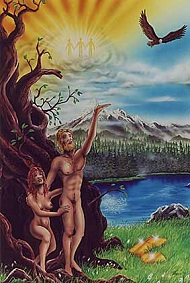
\includegraphics[scale=.7]{a20110608DreamingtheSameDream-img001.jpg} 
\end{wrapfigure}

Serrano was greatly influenced by Jung's idea of the Mysterium Coniunctionis, or the creation of the Androgyne. If every man and woman is a star, the spiritual and inner union of man and woman creates a new star. In a sense the woman surrenders her separate life, living on in the man in his consciousness. As Papan tells him:

\begin{quotex}
All that remains for me therefore is that other road of magical love which will deliver me over to you when I die. In this way I will continue to live, preserved in your memory. Do you realize that in a sense you are a kind of cemetery? You carry so many other around in you, and give them life through your memory of them.

\end{quotex}
By “dreaming the same dream” and sharing visions, the man and women are united. Her salvation comes from him, while she, embodying Wisdom or Sophia, reveals himself:

\begin{quotex}
When I came into her room I no longer spoke, but sat down in a wicker chair beside the window, and silently allowed her visions to pour over me, certain that hers and mine were the same, while all the time she looked through me as though I were a window.

\end{quotex}
Serrano, as a champion of the ascetic-heroic attitude, rejects the physical possession of the beloved:

\begin{quotex}
It should be known then that, in reality, the solution is to be able to bring Her back to life to resurrect Her within his soul.

\end{quotex}
Obviously, this refers back to \textbf{Kalacharaka Tradition} in Tibetan Buddhism. There are three levels of Tantra corresponding to the tripartite nature of man.

\begin{table}[h]\small\centering
\begin{tabular}{rp{17em}l}
\toprule
Karma mudra &
This involves a real female partner, part of the realm of desire. &
Body\\\midrule
Jnana mudra &
At this level, the Yogi creates an image in his imagination. The realm of form. &
Soul\\\midrule
Maha Mudra &
At this level, the Tantrika is formless, with no separate existence. &
Spirit\\\bottomrule
\end{tabular}
\end{table}

Karma mudra (physical woman) and jnana mudra (imaginary woman) are common occurences, available to anyone, with no discernible effect on any sort of gnosis or enlightenment. It is the practice of the Maha Mudra that interests us. In the first two levels, the woman is a privation to the man, while at the third the privation is overcome. The female element is absorbed into the man, creating a being superior to either of them separately.

Sophia, or the Virgin, is the World Process unfolding in our consciousness. As long as the Virgin is objectified, the World Process represents a privation to us, something outside us, beyond our command. It runs on its own. We represent this Process as horizontal, while the action of the Spirit is vertical. The separation and objectification limits the Power of Spirit. The male principle is Spirit (formless), the female principle is the flow of forms revealed in consciousness.

The task of the Yogi is to bring those principles in harmony, to “dream the same dream”. By ascetical and hermetic practices, he quiets the mind, to open a clearing in Being, where Spirit can act. The Virgin then is the perfect reflector of Spirit, revealing to him what He is. In this way, a new child is born\footnote{\url{https://www.meditationsonthetarot.com/the-word-is-made-flesh}}: the Androgyne, the Self, the Christ.



\flrightit{Posted on 2011-06-08 by Cologero }

\begin{center}* * *\end{center}

\begin{footnotesize}\begin{sffamily}



\texttt{Cologero on 2011-06-24 at 22:52 said: }

I found this rather odd story about “dreaming the same dream” in the Rolling Stone hit piece on Michelle Bachmann\footnote{\url{http://www.rollingstone.com/politics/news/michele-bachmanns-holy-war-20110622?page=3}}:

\begin{quotex}
Bachmann claimed that back in her college days, she was up one night praying with a female friend of hers when “the Lord gave each one of us the same, exact vision… It was a picture of me, marrying this man, in the valley where his parents have a farm in western Wisconsin.” Meanwhile, miles away, Marcus “was repairing a fence on the farm where he worked, and the Lord showed him in a vision that he was supposed to marry me.”

\end{quotex}
Leaving aside the unappealing content of her neo-Christianity, Bachmann illustrates the remnants of an archaic consciousness in the modern world: visions, communications with a god, destiny, and the obsession with the ties of family and religion. In contrast, the author represents the post-modern mind and there is, apparently, no point of contact between the two. Instead of an objective and dispassionate essay, he resorts to hysteria, a quality unbecoming in a man. For “those who know”, however, this is just another battle between fideists and post-modernists and is viewed dfferennntly. The post-modernist rejects every aspect of the archaic consciousness, while the fideist claims to hold a monopoly of every preternatual and supernatural manifestation in that consciousness.


\end{sffamily}\end{footnotesize}
